\label{appendix:Species}

\begin{table}[h]
\begin{center}
\begin{tabular}{|c|c|}
\hline
\multicolumn{2}{|c|}{\bf Primary}\\
\hline
{\bf Subspecies} & {\bf Uplifts/Clients }\\
\hline
\hline
\multicolumn{2}{|c|}{Humanity}\\
\hline
Dgn & Homo Sapiens Sapiens\\
Mishtali & Homo Sapiens Superioris\\
Purth & Home Sapiens Pluralis\\
Super Cetaceans & Homo Sapiens Cyberis\\
Super Simians & Homo Sapiens Suprahomo\\
& Homo Sapiens Cosmonatalis\\
\hline
\hline
\multicolumn{2}{|c|}{Rlaan}\\
\hline
Lmpl & Defender\\
Nuhln & Hybrid\\
Saahasayaay & Worker\\
\hline
\hline
\multicolumn{2}{|c|}{Aera}\\
\hline
Bzbr & \\
\hline
\hline
\multicolumn{2}{|c|}{Ancients}\\
\hline
Unknown & Various (at least 2 local) \\
\hline
\hline
\multicolumn{2}{|c|}{Those Who Have Only Names (TWHON)}\\
\hline
\hline
\multicolumn{2}{|c|}{Klk'k}\\
\hline
\hline
\multicolumn{2}{|c|}{Shmrn} \\ 
\hline
\hline
\multicolumn{2}{|c|}{Uln} \\
\hline
\hline
\multicolumn{2}{|c|}{Hoffman's blobs}\\
\hline
\end{tabular}
\caption{Relevant species of the UTCS time period}
\label{table:relevantspecies}
\end{center}
\end{table}

\section{Aera}

An intelligent centauroid species which developed on a misbegotten
hell of a jungle world, the Aera are oxygen-nitrogen breathers, with a
strong internal skeleton, smooth ashen-gray leathery skin, a decided
lack of psychiatric assistance for their obviously repressed
dissatisfaction with natural ecology and, at least according to the
Cult of the Devourer on Mishtal Seven, a flavor remarkably similar to
that of a human with a high protein diet, but only if both have been
served with a nice Chianti.

Unfortunately for the Aera, their region of the jump network offers no
known paths towards significant further expansion. To expand they must
go coreward, passing through Human or Rlaan controlled
systems. Requests to do so have been denied by both the relevant
parties of both species. Opting for another method, the Aera tried to
sneak a colony convoy through Rlaan space, but a lack of comprehension
of the Rlaan mentality regarding civilian casualties caused this ploy
to be not only a failure but a disaster, provoking the Rlaan into a
military response.

\subsection{Physical characteristics}

The Aera are a centauroid species measuring 2-3 meters in length from
the head to the end of the balancing tail, and 1 - 1.25 meters high at
the four leg- shoulders. The four stocky, sturdy running/gripping
limbs provide support, and the front two limbs end in three-digit
hands, with two fingers and an opposable thumb. When active, the upper
body bends up from the rest of the body just past the middle limbs at
about a sixty-degree angle, with the forelimbs sprouting from about
two thirds of the way up the upper body, and with the head bending
back down so as to be parallel with the main trunk and the
ground. Aera tend towards slim, muscular builds, and are usually both
quick and agile. They have two genders, each of which is similar in
appearance. Among the spacefaring races, the Aera have one of the
shorter natural lifespans. Prior to the advent of advanced life
extension technologies, it was as rare for an Aera to reach 60 years
of age as it was for a twentieth century human to reach 100.

The physical appearance of the Aera reflects upon their origins. The
Aera have a smooth, leathery skin not dissimilar in appearance to the
bark of a birch tree, with occasional yellowish patches reminiscent of
lichens. The hinged portion of the mouth is, in contrast to that of
terran species, the upper portion. The mobile portion of the mouth is
also notable in that it does not consist of a bony arch, and is
actually a solid bony plate. Inside this mouth are two rows of teeth,
the second moving forward to replace the first as they naturally fall
out, and a new second row is grown. The front teeth are razor sharp
and are obviously for tearing flesh, and the next sets of teeth are
likewise designed for the chewing of meat, but the rearmost few teeth
have grinding surfaces, allowing the consumption of nuts, seeds, and
other such vegetable matter. The corners of the mouth are usually
open, and provide the normal breathing route. When exerting itself, an
Aera will pull back its lips, increasing the size of the airway. The
wide, narrow eyes are almost universally a milky green, with wide,
narrow pupils, and are largish in size relative to the head. The eyes
are above the terminating point of the downward slant of the lipline,
but below the bony jaw plate. Just below the mouth, on each side of
the head, is a row of small pits that are used for
chemoreception. Beneath each eye is a kidney-shaped patch of lighter
skin that marks the location of a tympanum. On the underside of the
Aera head is a pair of organs, each capable of producing variable
amplitude, low frequency vibrations, which the Aera use to
communicate.

NOTE: depiction of head in Figure~\ref{fig:Aera-body} is non-canonical, picture otherwise highly informative:  

\begin{figure}
\begin{center}
\makebox[\textwidth][c]{
    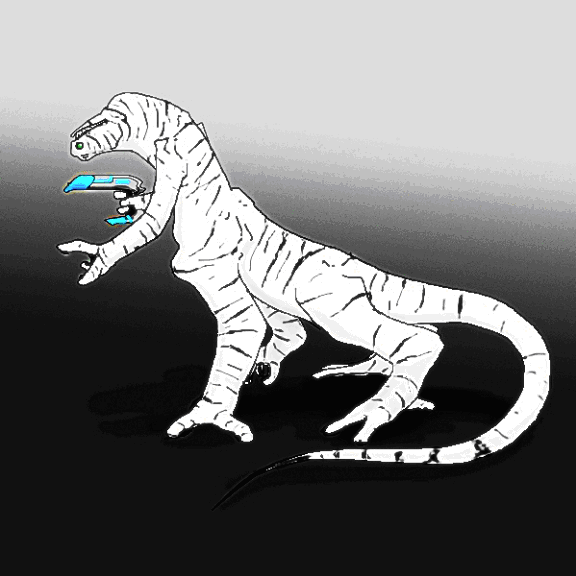
\includegraphics[width=\textwidth]{../images/Aera.png}
}
    \caption{Aeran. Head is non-canonical and should treated as such. Rest of body is a reasonably solid depiction.}
    \label{fig:Aera-body}
\end{center}
\end{figure}


\subsection{Habitat}
The Aera homeworld was, prior to changes imposed by the technological
advancement of the Aera, a nearly seasonless planet with an
oxygen-nitrogen-neon atmosphere, on whose surface were a single large
landmass and many large and small islands. The mainland was nearly
entirely covered with jungles and marshgroves, with only small belts
of more sparsely overgrown land on the northern and southern reaches
of the continent. The rich jungle land was home to all sort and manner
of parasites, predators, diseases, and competitors for food. It was in
this vast, dark jungle that the Aera arose into sentience, tool use,
and civilization.

\subsection{Culture}
Aera culture is highly organized and decidedly hierarchical, but in
the form of a meritocracy rather than an aristocracy. While what has
constituted merit has morphed over the millennia since the first Aera
tribes selected work crews to cut back the encroachments of the jungle
upon their early settlements, given the relative position of the
pre-technological Aera in their local food chain, there has long been
a favoring of cleverness and determination over raw strength. The
current social and vocational position of any Aera is immediately
indicated by the color and pattern of an individual's coverall. The
Aera are ruled by a subset of the highest caste, with membership in
the oligarchy changing whenever either an individual steps down, or a
third of the other members call for a member's replacement. New
members must be confirmed by two thirds of the current oligarchy. It
is much more common for members to voluntarily remove themselves from
power, believing themselves more useful elsewhere in society, than to
be cast out. An average stay in the oligarchy lasts a few Aera years.

The long struggle of the Aera against the erosion of their society at
the hands of the natural world has instilled in them a deep respect
for that which has enabled them to conquer their environment:
technology. Not only is the advancement of technology greeted without
fear, the social position of the artificer and the engineer is one
more greatly elevated than that seen in any pre-Diaspora human
society. What is feared is the unmastered and uncontrolled. Even after
the last war between Aera and Aera was fought, bringing the last of
the major islands under the control of the mainland, the Aera only
slightly relaxed their military investment. Perhaps in large part due
to their short lifespan, and the consequential rapid dying off of
adherents to old theories, science advanced quickly, and with the
understanding of their place in the universe came a belief that just
as they had been forced to fight back against the jungle to keep
themselves alive, so would they likely have to push back against all
that waited for them beyond their world. Thus, eight centuries ago the
Aera burst forth from their homeworld, not afraid, but determined that
nothing would stand between them and their indefinite existence.

{\bf Factions and Organizational Groups}
Listed below are noteworthy Aeran sub-factions and organizational groups: 
\begin{itemize}
\item Aeran Merchant Marine
\end{itemize}

\subsection{Religion}
The nature of the Aera homeworld never inspired much belief in any
sort of loving deity. What began as a collection of local deities
coalesced, through conquest by what was to be the dominant group on
the entire planet, into a single pair of entites, one force of
creation, and one of destruction, both abstract, and both uncaring. As
time progressed, and the Aera advanced, these entities progressively
lost entity status and drifted into the realm of spiritual
concepts. Becoming more self-centered in their exploration of
existence, destruction morphed into personal death, and creation into
species survival. Organized religious activity among the Aera, such as
it was, ceased centuries ago, but the impact on their culture of the
concepts of death and survival is still quite strong. Indeed, Aeran
mausoleums are said to be, quite possibly, the only pieces of Aeran
art that might ever be considered beautiful. The Aera respect death,
but value is placed on the accomplishments made in the face of one's
imminent demise. All Aera are cremated, and the repositories for such
remains are vast public works, filled with displays of the
accomplishments of those entombed within, those who contributed
greatly to the species being rewarded with physical space devoted to
listing their deeds, and the rest consigned to a rotating schedule of
intermittent holograms and access via terminal displays. It is in such
places that an Aera would go to ponder, in silence and solitude,
relenting briefly from the near tireless schedule of a short-lived
species, the nature of its existence.

\subsection{Miscellaneous}
The Aera use a redundant numbering scheme:
Radix 3, digits drawn from the set of values {-2,-1,0,1,2} 

\section{Ancients}

\subsection{Physical characteristics}
There are precious few preserved remains of either species A or B
(especially B), so knowledge of their physiology is pieced together
from various, sometimes conflicting sources.

{\bf Species A}

Species A were moderately sized beings, between 1 - 3 meters in height, and no more than 2 meters in diameter. 

{\bf Species B}

Species B were smaller beings, no more than a meter wide, high, or thick. 


\subsection{Habitat}
The native habitats of these creatures are unknown. Given the nature
of the planets they settled, it can be assumed that they were
carbon-based lifeforms, and that at least of one of the two was an
oxygen breather.

\subsection{Culture}
Beyond their technological advancement, little is known. 

Excerpt from "A Brief History in Time and Space" 

"While there is much contention about the nature of the predecessors
of the Ancients, the Ancients themselves left enough rubble strewn
around the galactic arm to convince even a fairly hardened skeptic of
their having dwelled in these parts. The Ancients appear to have been
made up of at least two major species groups, and interacted with at
least three others, albeit it is not known whether these were client
species, or contemporaries from another part of the galaxy. Their
reign over this region lasted until about 1 to 2 million years ago,
whereupon they rapidly ceased to be present. There is a wealth of
evidence that severe infighting played some part in the destruction of
the Ancients, but, assuming there were victors in such a conflict,
little is known of what became of them.

The best source of such evidence, however limited, is the Uln
homeworld. While they are quite sensitive about the subject, the
widely held belief among the major races is that the Uln are the
descendants of the Ancient's equivalents of lab monkeys. The Uln
culture sprang up among the remains of a sprawling set of Ancient
structures... if they hadn't been so ill prepared for the gifts they
unintentionally received, they would have conquered the entire
arm. Fortunately for the aspirations of dominance held by other
species, the Uln were decidedly unprepared. Indeed, they spent so much
time blowing each other up with weapons they didn't entirely control
that it is a wonder that either they or the ruins on their planet
still survive.  The ruins, however, did not escape unscathed from the
genesis of the Uln culture. While assuredly the largest known source
of information on the Ancients, the ruins deliver little coherent
information about many key aspects of the Ancients' existences,
largely due to vast portions of many buildings having been turned to
dust."

To clarify, the statement about the Uln possibly having been able to
conquer the arm is contingent upon them NOT having blown most of the
ruins up, along with the devices they were using to blow each other
up, and large portions of their own species. No superweapons as such
are known to be currently possessed by the Uln. The Uln are in
possession of one particularly impressive piece of Ancient technology
(what is known as the Sul-Gatwa high castle), but it's potential is
effectively limited to the defense of their homeworld. However, even
as heavily damaged as the finds on the Uln world are, they remain the
best source for archeological research, and research visas remain a
large part of the Uln economy.

Why would this blasted planet be the best source of artifacts?
Because, unlike most of the planets that seem to have been inhabited
by the Ancients, it didn't have it's entire surface slagged, get
broken into a debris field of billions of pieces of rock, or become
pockmarked by craters implying assault equivalent to prolonged
planetary bombardment by 500Km wide asteroids.

Despite this, the occaisional piece of debris is found in such
places. However, the only officially reported finds of
fully-functioning Ancient technology have been the nano-plague and
various minor finds on the Uln homeworld.

The largest known piece of Ancient technology is the Sul-Gatwa high
castle. Whether or not it is technically functional is a matter of
some scholarly contention - the object is a slagged chunk of some
small moon sized ship or station. No systems appear to be remotely
functioning. However, what information has been declassified by the
Uln Royal Ingatwa fleet and confirmed via espionage implies that the
structure is so dense that it should have collapsed under its own
gravity into a solid mass - however, as the material that the high
castle is composed of defies the best efforts of science to explain or
duplicate (it has been jokingly dubbed "unobtainium") it could just be
some intrinsic property of the material and not evidence of
functioning gravitics. While the high castle has none of it's original
equipment and is, in essence a giant chuck of debris in orbit around
the Uln homeworld, every indication is that it retains the potential
to absorb absurd amounts of damage, and, as such, the centuries that
the Uln have spent arming it with their own weapons have made it the
most formidable planetary defense station known to exist. Its
existence, the threat of the Uln destroying what remains of the
Ancient artifacts, and general opinion that any of the major powers
could pen the Uln into their home system if necessary are believed to
be the primary factors responsible for the Uln remaining independant
entities.

Small fragments of Ancient technology, even completely non-functional,
fetch a fair price at any research facility or university
planet. Functional pieces of Ancient technology, even if relatively
useless, are of exceptional value, and it is not unheard of for
persons to attempt to make a career out of artifact prospecting,
subsisting on the rewards from finding small pieces of debris while
waiting for the big catch of working Ancient tech. However, as time
progresses, the easier pickings have already been scavenged, and
exploration of progressively more hostile environments has become
necessary to sustain the trickle of finds.

\section{Bzbr}

The Bzbr are a psuedo-reptilian species found on a jungle planet by
the Aera early in their expansion. The discovery of organized alien
intelligent life, even if harmless in it's neolithic state, furthered
Aera convictions about the dangers of the universe, even as they
worked to co-opt the Bzbr.

\subsection{Physical characteristics}
A Bzbr most closely resembles a jungle-green, copper-highlighted
1.5-meter long, ten-legged, arboreal reptilian with a nearly meter
long prehensile tail. Each limb has four segments, the fourth being
the hand/foot equivalent. The rear six legs are built for jumping, and
are used only for locomotion, the two underslung short arms primarily
for food manipulation, and the two forward inline limbs primarily for
gripping branches or other such objects, arching upwards and forward
from the rest of the body, in contrast to the other inline limbs,
which proceed upward and outward from the torso. Lacking vocal cords,
the Bzbr communicate in a simple language consisting of varied buzzing
tones produced by rubbing their feeder limbs together and motions of
the gripping limbs.

The Bzbr have three genders, breeder, broodherd, and
gatherer. Gatherers are the most common gender, and conduct all
hunting activities. Breeders are smaller than the gatherers, and
forage close to the nest area for roots and nest building material. In
far smaller number than the breeders or gatherers are the broodherds,
larger, stronger, sterile, and existing solely to protect the young
and territory of their sisters. Normal Bzbr nest groupings number in
the few dozens of adults. Bzbr are exceptionally short lived, living
only 35 - 40 years, even with modern medical technologies, but, given
their small size, this is not entirely unexpected.

\subsection{Habitat}
A world of jungle islands, spontaneous firestorms due to the high
oxygen content of the atmosphere, and extreme seasonal weather shifts,
the Bzbr homeworld can be safely considered unpleasant to all of the
known spacefaring races.

\subsection{Culture}
Adopted by the Aera out of some combination of pity and sympathy for
similar jungle origins, the Bzbr were pulled straight from the stone
age to the FTL age. Adapting about as well as can be expected to this
rapid change, many Bzbr simply went insane trying to adapt, but after
a few generations, the Bzbr had come to accept the new reality, even
if they were, due to rather much less than genius level average
intelligence, ill equipped to fully understand the full complexity of
it. Although not particularly bright or creative, the Bzbr are
actually quite good at both remembering and following instructions,
and have come to be used in various Aera space construction projects,
where they are valued for their ability to deftly maneuver in small
spaces and to leap from girder to girder. Bzbr, are, however, never
seen far from their Aera Patrons, as they are quite lost without
them. The Bzbr still, to some great degree, see the Aera as messengers
of the gods, having delivered them from the horrors of their world,
even if they know the Aera to be both mortal and fallible.

\subsection{Religion}
Though the Aera have attempted to convince them to do otherwise, the
Bzbr engage in hero-worship of the Aera. A majority of the Bzbr are
convinced that the actions taken in this universe play out in other
planes where the great nest of all life is threatened by chaos. They
believe that the Aera, by having brought greater order to their lives,
make them all great warriors in the other planes.

\subsection{Miscellaneous}
Bzbr use Aeran numbers. 

\section{Dgn}

The Dgn, like their brethren the Shmrn, are the descendants of a joint
Shaper and Lightbearer uplifting program begun with dextrous, tool
using, but pre-civilized saltwater marsh dwellers. The Dgn are the
branch cultivated by the Shapers and remain an integrated servant
class in Shaper society.

\subsection{Physical characteristics}
See images ~\ref{fig:Dgn-body} for bodyplan and ~\ref{fig:Dgn-motion} for locomotion (the Avian style is closest): 

\begin{figure}
\begin{center}
\makebox[\textwidth][c]{
    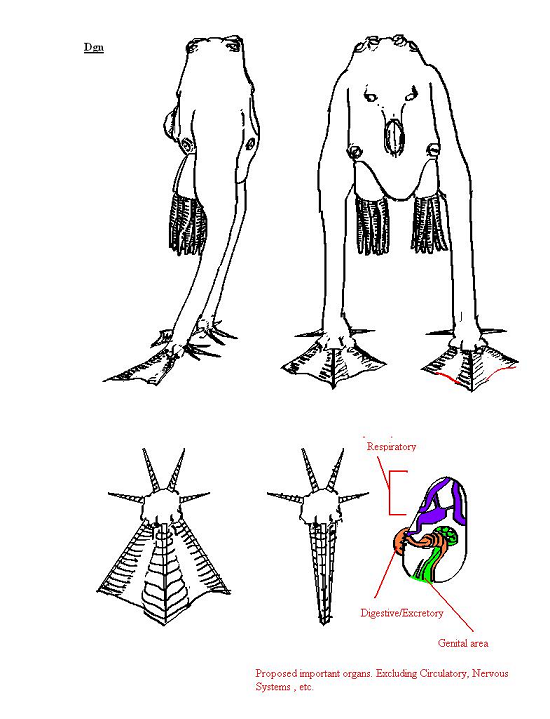
\includegraphics[width=0.95\textwidth]{../images/Dgn-body.png}
}
    \caption{Dgn body-plan}
    \label{fig:Dgn-body}
\end{center}
\end{figure}

\begin{figure}
\begin{center}
\makebox[\textwidth][c]{
    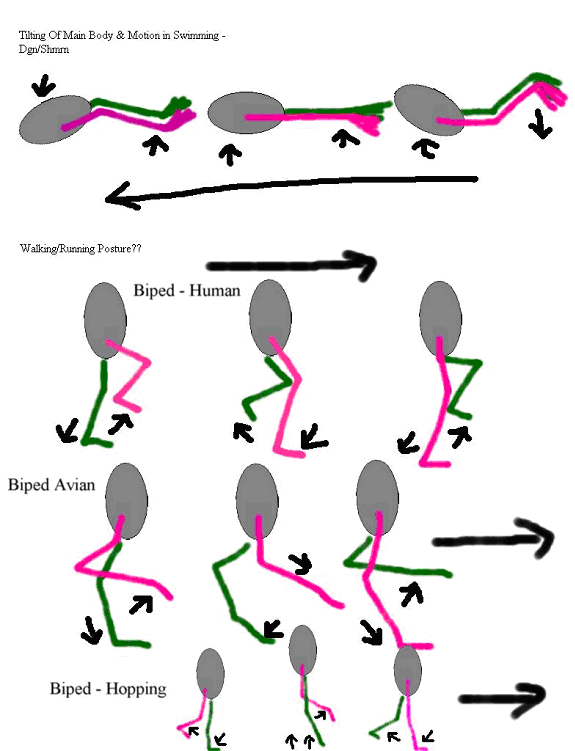
\includegraphics[width=0.95\textwidth]{../images/Dgn-motion.png}
}
    \caption{Dgn locomotion on land and in water}
    \label{fig:Dgn-motion}
\end{center}
\end{figure}



See Also: Shmrn (~\ref{subsec:Shmrn-species})

Through genetic engineering their life expectancy has been extended to over 50 years. 

\subsection{Habitat}

The Dgn can breathe in both atmospheric and aquatic conditions,
provided that there is sufficient oxygen dissolved in the water. They
do, however, require either a humid land environment, or frequent
re-wetting to keep both their skin and breathing orifices from drying
out. The native Dgn habitat ranged from coastal saltwater marsh-land
to tidal flats and into the coastal shallows themselves.

\subsection{Culture}

What native culture existed among the pre-modified Dgn has been
greatly altered. Bred for servitude, the Dgn are not greatly renowned
for intellectual achievements. The Dgn exist as a servant race for the
Shapers, working on nearly all Shaper aquatic projects, and filling
other unwanted roles in society. The one noted exception to this rule
is the use of Dgn as medical assistants in Shaper hospitals, where
their dexterity has proved them faster than humans at prepping the
injured for surgery. While the rights of the Dgn are well defined by
the Shapers, and abuse is not at all tolerated, their rights are not
the same as those of the Shapers, and if the Dgn are to be considered
citizens of the Shaper political body, then they are, at best, second
class citizens. The Shapers have built them to not be overly concerned
about this (the Shapers having had a different vision of what they
desired from their uplift than the Lightbearers, who were more
concerned with continued evidencing of their believed and beloved
superiority over lesser species). One cannot say that the Dgn are
entirely pleased with their position, but neither can one say that
there is fertile ground for revolt, as the Dgn do not seem to possess
within them a particular desire to be forced to decide their own
destinies. As the Dgn do not complain and the Shapers do not overtly
or actively seek to mistreat the Dgn, their freedom is something
sought after by activist groups rather than brought about by an armed
foreign entity.

\subsection{Religion}

Whatever glimmerings of disorganized religous beliefs they may have
had as more simple creatures have been lost. Currently prohibited from
engaging in organized religious activities due to historic fostering
of undesired solidarity.

\subsection{Miscellaneous}
Dgn use Human numbers. 

\section{Hoffman's blobs}

Hoffman's blobs are seemingly non-sentient creatures living in the
void of space. They were discovered by Burno Hoffman in the Barnard's
Star system.

\subsection{Physical characteristics}
Very little is known of those bizzare interstellar beings. The last
sighting has been in the Galileo system. Scientists are now flocking
to study these creatures before they leave, attempting to determine
how it is that they are able to sustain themselves in the void of
space. Observations suggest their size varying greatly, with the
largest individuals proving as large as a space cruiser, and the
smallest only the size of a shuttlecraft. It is uncleaer whether these
differences are attributable to age or polymorphism. The creatures
appear to primarily be drifters, but are capable of some acceleration.

\subsection{Habitat}
Hoffman's blobs live in the void of space. Since they were discovered
there have been six sightings of them, most recently in the Galileo
system.

\subsection{Culture}
There has not been any exhaustive research on the behavior of
Hoffman's blobs yet. From previous observations, it appears they
travel in flocks of about a dozen units.

\section{Humanity}

Table~\ref{table:relevantspecies} shows the relevant species in the UTCS time period and notes their organizational relations. FIXME (placeholder)

\begin{itemize}
\item	Homo Sapiens Sapiens (Faction with highest population percentage: Purists) 
\item	Homo Sapiens Superioris (Faction with highest population percentage: Shapers) 
\item	Homo Sapiens Cyberis (Faction with highest population percentage: Mechanists) 
\item	Homo Sapiens Pluralis (Faction with highest population percentage: Andolians) 
\item	Homo Sapiens Suprahomo (defunct) 
\item	Homo Sapiens Cosmonatalis (Faction with highest population percentage: Spaceborn) 
\end{itemize}
\subsection{Physical characteristics}
\begin{itemize}
\item Homo Sapiens Sapiens
\index{Homo Sapiens!Species info}
\index{Homo Sapiens!Homo Sapiens Sapiens}

Although small changes have occurred over the millenia, a great
percentage of the human population remains without intentional genetic
or physical modification, and thus remains not too far removed from
the humans of more ancient history. Whether through simple lack of
resources, lack of desire, or rejection of change, Homo Sapiens
Sapiens, unmodified except for the genetic drifts incurred over
centuries of colonization, remains the most populous of the human
subspecies.

\item Homo Sapiens Superioris
\index{Shaper!Species info}
\index{Homo Sapiens!Homo Sapiens Superioris|see {Shaper}}

Many eugenics programs have been launched in human history, but none
have been so successful. The path of self-affected evolution via
active genetic redesign has lead to a strain of humanity stronger,
more durable, more resistant to disease and injury, of higher average
intelligence, enjoying longer life-spans, and possessing keener
senses.  Assuming that the universally ink-black UV-resistant skin and
complete lack of any hair other than the signature blue-white
eye-brows is not disconcerting, any Superioris is almost certain to be
considered physically beautiful, but it takes some experience to
discern one Superioris from another. However, these benefits come at
the cost of much higher sustanence requirements, and a tremendous
narrowing of diversity.

\item Homo Sapiens Cyberis
\index{Mechanist!Species info}
\index{Homo Sapiens!Homo Sapiens Cyberis|see {Mechanist}}

Having replaced many of their body parts with mechanical equivalents,
or having forgone any pretense of human form, these cyborgs cover a
diverse and vibrant set of body types. Those with total body
replacement can usually pass anything short of close inspection if
they're willing to deal with maintenance of a synthetic flesh
exterior. If the goal is, as is often the case, to adapt the body to
the demands of work or habitat, anything from mining attachments to
full strength-enhancing endoskeletons could be an integral part of the
form. Locomotion seen to date ranges from bipedal to poly-pedal,
tracked, wheeled, or even sets of thrusters. In addition, this sort of
technical enhancement may provide the ability to extend one's lifespan
indefinitely if the base neurological systems have already been
altered to be non-senescent (provided one has access to regular
maintenance service). However, no matter how modified they may be, at
the least, portions of their brains and nervous systems remain.  While
communities of such modified humans exist on the worlds of many
factions, the Mechanist faction is the only full-fledged meme-group
centered upon the post-flesh goals of Homo Sapiens Cyberis.

\item Homo Sapiens Pluralis
\index{Andolian!Species info}
\index{Homo Sapiens!Homo Sapiens Pluralis|see{Andolian}}

While various communities have arisen that rely upon linked
existences, none save the Andolians have sufficiently differentiated
themselves en masse from the rest of humanity to be a discernable
grouping. Implanted at birth with hardware that allows data-net access
and an array of almost constantly transmitting sensors, a permanently
linked existence has rendered this strain of humanity notably
different in culture and mentality from all other strains.  While
every Pluralis retains its individuality, each is awash in a similarly
accessible sea of information. Culling from the group of those not
capable of entering into such an existence combined with a willingness
to engage in limited crafting of offspring has also lead to small but
noticeable genetic drift over the past 800 years. Implantation is
universal, and the use of synthetic or mechanically enhanced body
modifications is not uncommon, but the desire for total body
replacement present in the Cyberis strain is absent.  The linked
existence and general cultural proclivities of the Andolians have
brought them to near unity on their religious doctrine. While an
Andolian would refer to his/herself as a devout skeptic existing in
the absence of proof of the metaphysical, many others find it simpler
to call them Atheists.  While not overly concerned with improving the
physical form, health-related genetic traits deemed undesireable have
been recorded and then excised from the gene pool. When isolated for
long periods of time from any data-net, Pluralis individuals often
experience pronounced withdrawal symptoms, earning them the nickname
"Link-Junkies".

\item Homo Sapiens Suprahomo (Lightbearers) (Nearly Extinct) 
\index{Lightbearers!Species info}
\index{Homo Sapiens!Homo Sapiens Suprahomo|see {Lightbearers}}

One of the earlier factions to aggressively expand outward in the FTL
era were the Lightbearers, a meme-group built around the development
of a supra-human race. Believing the human form to be the sacred
forefront of evolution in the entire galaxy, they sought to claim the
place of their distilled and purified strain at the throne of all
sentients.

\item Homo Sapiens Cosmonatalis
\index{Spaceborn!Species info}
\index{Homo Sapiens!Homo Sapiens Cosmonatalis|see{Spaceborn}}

Crafted as a slave race by the now defunct Light-Bearer faction, the
Spaceborn, as they are commonly referred, remain frail and
over-specialized, incapable of surviving in planetary
environments. Instead, as they were designed, they spend their entire
lives in micro-gravity. The Spaceborn have a unique cardiovascular
system superbly tuned to life outside of a gravity well.  Their bone
structure, however, is a less cheery affair, and the Spaceborn, though
not suffering the degenerative effects of planetborn entities in
prolonged micro-gravity, never had much durability in the first place
and are weaker and more easily injured. They are almost universally
tall, lanky, and flexible, and all are possessed of a rather pallid
complexion tending toward a slight reddishness. Spaceborn frequently
begin developing severe medical problems between the age of 60-80
Earth years, giving them a somewhat shorter life expectancy than that
of the other subspecies.  Almost all Spaceborn live in habitats
situated in Andolian Protectorate space, having relocated from
Light-Bearer space after liberation from that faction.
\end{itemize}

\subsection{Habitat}

Originating on the third world of the Sol system, all variants of
humanity, even Homo Sapiens Cyberis, are most comfortable in
Oxygen-Nitrogen atmospheres, and temperatures not overly distant from
294 Kelvin.

\subsection{Culture}
Listed below are links to noteworthy human Meme-groups, organizations,
and governments:

FIXME 

\subsection{Religion}
Among the most mixed and varied in the known galaxy, running the gamut
from atheists to zealots. Refer to the individual groups for more
information.

\subsection{Miscellaneous}
Base 10. 

\section{Klk'k}
FIXME 

 
One of only five extant species to have achieved some measure of
space-flight prior to contact with other sentients, the Klk'k had what
can be readily argued as the worst first-contact experience on
record. Although the Andolian backed Ktah Restoration Project did much
to stem and repair the damage caused by the Lightbearers during their
occupation of Ktah, nearly a quarter of the Klk'k species were killed
by the Lightbearers, the majority of the deaths stemming from the
Lightbearers retargetting their fusion-tipped anti-orbital defense
missiles for ground impact and launching all batteries in a
scorched-earth response to the Hoshino Uprising. While the
laser-induced fusion warheads were exceptionally clean in the
radiologic sense, the scale of the bombardment was such that there
remain a number of areas of Ktah which have not fully recovered, even
at more than two centuries remove.

Currently, almost all Klk'k are citizens of the Andolian
Protectorate. While the Klk'k are self-governing over their own
colonies on domestic matters, with a government centered in Ktah, they
defer to the Andolians on external affairs. A significant minority of
the Klk'k population have become active adherents to the Andolian
meme-group, living integrated existences networked into surrounding
Andolian populations. Several mixed-species colonies featuring both
Humans and Klk'k exist, and there is both a human and Klk'k presence
on all Purth worlds.


\subsection{Physical characteristics}
average height range 4.5 to 5.5 feet (in meters?)

long, largish feet, reverse jointed knees, large easily splayed hips,
excellent jumpers, thick, disproportionally long, muscular legs in
proportion to generally much skinnier tops

wide, short, fair lengthed, back-bottom flanging head, with back
facing nostrils at the rear base between neck and jawbone

jaw is wider than head on each side. because of angle, more teeth on
bottom jaw than on top, bottom jaw teeth face slightly in, top jaw
teeth face slightly out

mouth contains 2 tongues. has no connection to air passageway. has
resonant "click" cavity in front top of mouth, behind and below the
rear of the bone ridges forming the eye sockets

eyes are large and wide set, and the sockets prononouced in their
bonyness

ears, such as they are, are 2 long curved ovoids, extending forward
from just behind and below the top of the jaw joint to somewhat even
with the top of the jaw joint and in front of the joint.  Mostly flush
with the skull, each ear is a series of cartilige-analog ridges
protruding slightly out from the side of the head to focus sound into
a central shallow curved trough, the bottom of which has numerous tiny
folds of hair-lined skin atop a drum

See additional discussion (later in document)

Figures ~\ref{fig:Klk'k-body-front},~\ref{fig:Klk'k-body-side}, and~\ref{fig:Klk'k-body-head} are poorly drawn sketches of the basic Klk'k body plan. Though
they show the general outlines, they are inconsistent as to whether
they are showing skeletal/muscular/etc. structures and details (to be
taken as rough guidance only - not canonical due to poor
implementation of desired visible outcomes (i.e. jacks can't draw
worth a damn))

\begin{figure}
\begin{center}
\makebox[\textwidth][c]{
    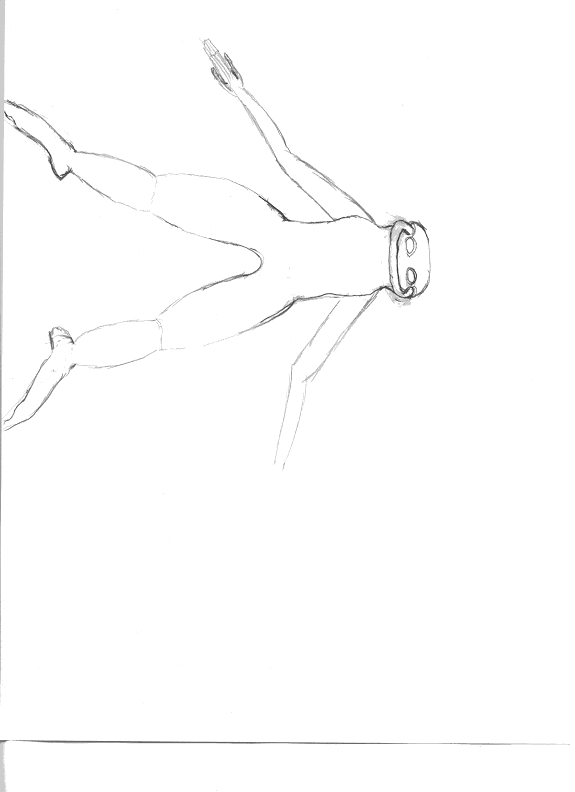
\includegraphics[width=0.75\textwidth]{../images/Klk'k-bodyplan-front.png}
}
    \caption{Basic Klk'k body plan (front)}
    \label{fig:Klk'k-body-front}
\end{center}
\end{figure}
\begin{figure}
\begin{center}
\makebox[\textwidth][c]{
    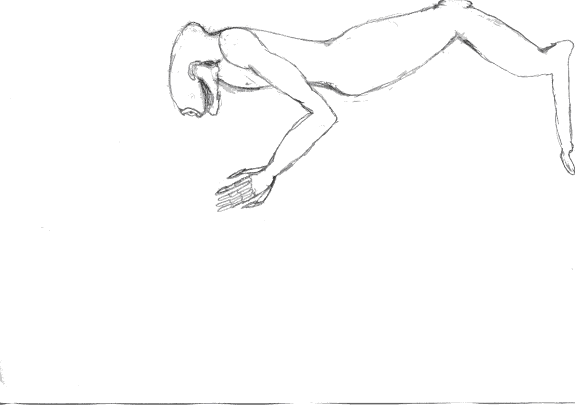
\includegraphics[width=\textwidth]{../images/Klk'k-bodyplan-side.png}
}
    \caption{Basic Klk'k body plan (side)}
    \label{fig:Klk'k-body-side}
\end{center}
\end{figure}
\begin{figure}
\begin{center}
\makebox[\textwidth][c]{
    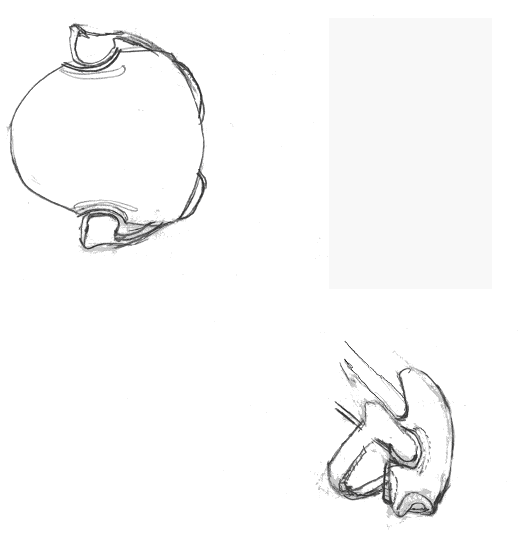
\includegraphics[width=\textwidth]{../images/Klk'k-bodyplan-head.png}
}
    \caption{Basic skeletal structure of Klk'k head}
    \label{fig:Klk'k-body-head}
\end{center}
\end{figure}

The most anthropoid of the sentient species that humanity has
encountered (admittedly, two arms, two legs, two eyes, one head is
enough to place them ahead of most others), the Klk'k are nonetheless
notably alien in nature. Bipedal, with bilateral symmetry, the Klk'k
stand 1.3 to 1.5 meters tall on two splayed, reverse-jointed, muscular
legs, balancing on extremely elongated feet. Two arms,
disproportionately long by human standards, drape down from the
shoulders, each ending in a hand with four wiry fingers and two
thumbs, one on each side. The thumbs have something resembling nails,
while the rest of the fingers terminate with a hard, leathery, callus
covering the top and front, the finger-tips remaining fleshier. Klk'k
toes terminate in short, thick, blunt, stubby claws far more useful
for climbing than for tearing. The Klk'k head is wide and somewhat
squat in comparison to its breadth, being noticeably wider, at the
bottom, than the Klk'k neck. The Klk'k face features two large eyes
and a mouth that opens most of the way back to the jaw hinge. The
jawbone continues in an outward direction somewhat as it goes down
from the skull, further accentuating the width of the Klk'k head. The
Klk'k air passageways and digestive tract are separated. Breathing is
performed through two rear-facing nasal openings, one on each side of
the back of the head, situated behind and under the jawbone
attachment, opening where the head curves back to meet the neck. The
two eye sockets are protected by pronounced brow ridges. Inside the
mouth is a resonating click cavity, and two tongues. Klk'k have
several smaller, sharp, front teeth, and a smaller number of larger
grinding teeth, present only at the back of the mouth. Klk'k ears have
minimal external presence compared to human ears, presenting
themselves primarily as a furrow curving back and down along each side
of the Klk'k skull. The ears are water-tight, and Klk'k underwater
hearing is significantly superior to that of humans.

Klk'k are hairless, and the skin tends toward a swampy, uneven
green-brown, excepting the secondary sexual characteristics which
express themselves as thin, rosy-to-purplish highlights on the sides
of the head, hips, wrists, and ankles. Skin tends to be smooth, and
slightly leathery in texture, but a substantial layer of subcutaneous
fat keeps it from being hard to the touch. Both sexual and excretory
organs are positioned similarly to those of humans, at the posterior
of the torso. The Klk'k have two genders, the female of the species
tending to be the larger of the two, and distinguishable, among the
adult population, by the presence of more purple, rather than rosy,
highlights. Distinguishing between the genders of Klk'k children is a
more difficult task for the untrained human eye.

Klk'k have single fetus (with few exceptions) internal pregnancies,
and exceptionally long gestation periods. The later stages of the
pregnancy are extremely debilitating to the mother, eventually leaving
her nearly immobile as the fetus grows to increasing size and the
birthing blister migrates progressively closer to the
surface. However, at birth, the newborn Klk'k can already walk, swim,
and consume normal food.

Klk'k speech is produced primarily as a combination of vowels and
tones from the nasal airways and clicks from the tongues and
resonating chamber. Manipulation of the closures to the nasal airways
also produce a smaller number of consonants. The tonal nature of each
airway is independent, and harmonics have semantic and syntactic
meanings in most of the native Klk'k languages. The iconic Klk'k nasal
horn takes explicit advantage of the dual-tonal capabilities of the
Klk'k. Some human observers have likened Klk'k speech to listening to
a pair of Hawaiians having an animated conversation with a pair of
Khoisan, but most real xeno-linguists attempt to discourage such
simplistic comparisons as more misleading than informative. "Klk'k" is
itself an anthropic transliteration of their word for themselves,
likewise for Ktah, and Tk'latl, etc. As the Klk'k have proven far more
adept at understanding spoken human tongues, than the reverse, even if
they cannot produce the full range of human sounds, the anthropic
forms have become accepted standards, rather than requiring all humans
to utilize translator devices to refer to anything of Klk'k
origin. Klk'k living or traveling among humans tend to equip
themselves with vocalizing augmentation devices that fill in the
missing gaps in their ability to emulate human speech.

\subsection{Habitat}
Ktah is a warm, wet world with an Oxygen-Nitrogen atmosphere and vast
open stretches of ocean surrounding the two major continental
bodies. The Klk'k originated on the smaller of the two continents,
developing amidst the seemingly endless criss-cross of rivers and
bayous that dominate it. Though not amphibious, the Klk'k are quite at
home in the water, being excellent swimmers.

\subsection{Culture}
Humor plays a deep and intrinsic role in Klk'k culture, far beyond
that in any human one. While the Klk'k equivalents of humor and even
laughter have strong similarities to their human counterparts, the
situational appropriateness of humor is viewed quite
differently. There are few things that necessitate a somber decorum
for a Klk'k - they would see nothing inappropriate about joking and
laughing at someone's deathbed, funeral, execution, summit, board
meeting, intelligence briefing, etc. Indeed, quite the opposite is
true. Even war and combat are not seen as entirely serious realms --
there are numerous Klk'k stories involving tales of foes refraining
from death blows because each was waiting for the punchline of the
other's joke. Humor is also seen as appropriate in public actions,
officials, and governmental entities. In one particularly long-running
tradition, legislation is frequently put forward to change the Klk'k
anthem for the duration of a visiting dignitaries arrival in order to
make atrocious puns.

Being unable to find or generate humor in one's situation is a sign,
in a Klk'k, of a present or imminent psychosis, if often only a
temporary one. Klk'k can be riled to an indignant rage that, if short
lived, is still disturbing in its intensity. In Klk'k martial arts,
such as Amakakt, sparring contestants are often required to keep a
running dialog of humorous insults. If one of the combatants becomes
noticeably silent, the match is suspended, as it is a sign that
control has been lost, and the onset of rage may be approaching.

The basic Klk'k family unit is the the bond-set, based around a
mutually polyamorous clique arrangement. A bond-set usually consists
of 3-6 adult Klk'k and their assorted children, with the parentage of
the children coming from any arbitrary pairing within the
bond-set. Bond-sets consisting of only 2 Klk'k, save as a result of
the death of additional members, or as an initial state, are
considered strange, and their members potentially dysfunctional if
that arrangement persists. Bond-sets will continue to grow over time
by mutual interest in inclusion until they reach a steady point for
the individuals involved. Bond-sets with more than 6 members exist,
but are rare, as finding large numbers of co-interested partners is a
non-trivial task. Four members is the median expectation, and many
bond-sets of three partners will delay having children until a fourth
has joined. Some researchers believe the extended size of the basic
family unit to have roots stemming from the degree to which the later
stages of Klk'k pregnancies are completely incapacitating, leading to
a need for a larger supporting family unit.
\begin{itemize}
\item Bond-set Naming Conventions

The dominant culture for quite some time has used a strict two-name
scheme. When a bond-set is formed, the members choose a name for
themselves, and that is the bond-set name for those children raised by
that set. If the set changes, through addition, the name may be
changed or it may be kept, but the children will retain the old name,
unless very young. If the set changes through attrition, the name does
not change in order to honor what was, even if it is no more. One is
known by one's bond-set name (the name of those who raised you) and
your personal name, usually given in that order, thus Klk'k names are
not lineage tracing beyond a single generation.

\item Clothing and Ornamentation

Nudity was not a big deal in any notable pre-contact Klk'k culture,
and continues to be of little concern except among those Klk'k
visiting human worlds obsessed with particularly archaic
taboos. Common Klk'k coverings are as much practical and protective as
shielding from the public eye, featuring pockets, belts, places to put
or hang things, footwear, and isolated pieces to prevent scrapes and
scratches to various sensitive areas.

Klk'k style uni-gender semi-formalwear tends to be variants on a
loose, sleeveless (there is fabric straight from shoulder to neck, but
no collar), single-piece garment that runs completely flat across the
front, tapers slightly out from waist down and is slit in the back
somewhat below the end of the torso (the rear opening being convenient
for the Klk'k as their legs bend opposite those of
humans). Ornateness, except in extremely formal clothing, is highly
restrained, with patterns being limited to the edges and waist area,
running in thin seams around the garment. The prime regions of Ktah
are quite humid, and ostentatious layering would not have been
comfortable. Those looking for a more vibrant appearance tend to do so
with body paints on exposed skin rather than additional
clothing. Informal Klk'k clothing tends towards a short, loose skirt,
with tops, if any, varying by region.

There is also specific clothing to show respect, show allegiance, and
traditional body-paintings and tattoos. In particular, Amakakt tattoos
are expected among those practicing the martial art. A Tk'latl is
tattooed on the upper left topforearm/shoulder area, with annotations
denoting rank and record in Amakakt (the martial art heavily featuring
said Tk'latl). The ranking is above the Tk'latl, and consists of a
series of vertical bars of different color, denoting increasing ranks
attained, from left to right. A history of the matches is recorded in
colors corresponding to the rank of the opponents, and lies below the
Tk'latl, with vetical bars for victories and horizontal bars for
defeats.

Klk'k members of the Simons are known to frequently sport dynamic
tattoos, making their membership explicit when desired and hidden when
inconvenient.
\end{itemize}
\subsection{Religion}
The Klk'k frowned intensely upon organized religion even before they
settled under the wing of the Andolians. Klk'k history had been rife
enough with false prophecies and self serving church-like
establishments (including a theocracy that once dominated much of
Ktah) that the Klk'k analog to the Enlightenment had been rather total
in its sweeping reforms. Klk'k culture, however, has a long history of
veneration of ancestors, which continues in various ritualized forms
of behavior. There is no belief among the Klk'k that the deceased may
be contacted, nor is there any particular spiritual nature to the
reverence for those who came before, merely the conviction that it is
one's duty to honor the fact that, without them, one would not be.

\subsection{Miscellaneous}
Base 12, with numeral set derived from 2x2 entries in (2,3) double
base number system.

\section{Lmpl}

\subsection{Physical characteristics}
See Figure~\ref{fig:Lmpl} for image of a
Lmpl. Figure~\ref{fig:Lmpl-working} shows a Lmpl performing various
tasks.

\begin{figure}
\begin{center}
\makebox[\textwidth][c]{
    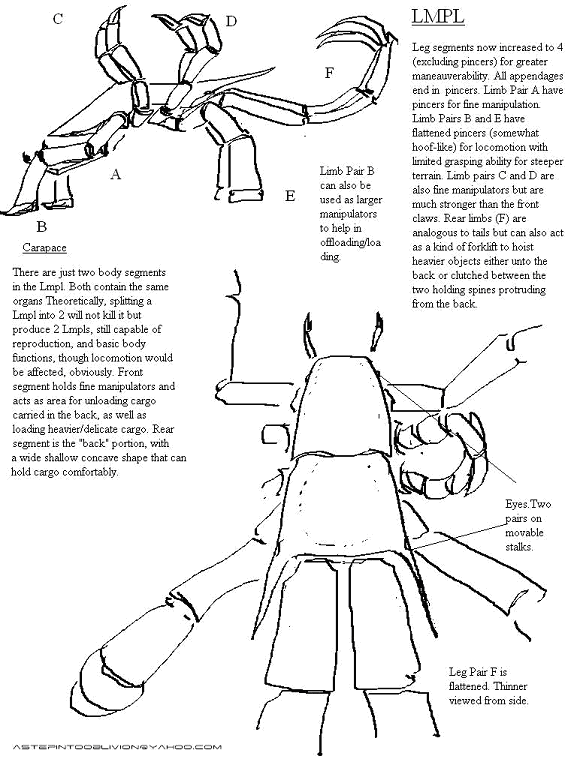
\includegraphics[width=0.75\textwidth]{../images/Lmpl.png}
}
    \caption{Image of a Lmpl}
    \label{fig:Lmpl}
\end{center}
\end{figure}
\begin{figure}
\begin{center}
\makebox[\textwidth][c]{
    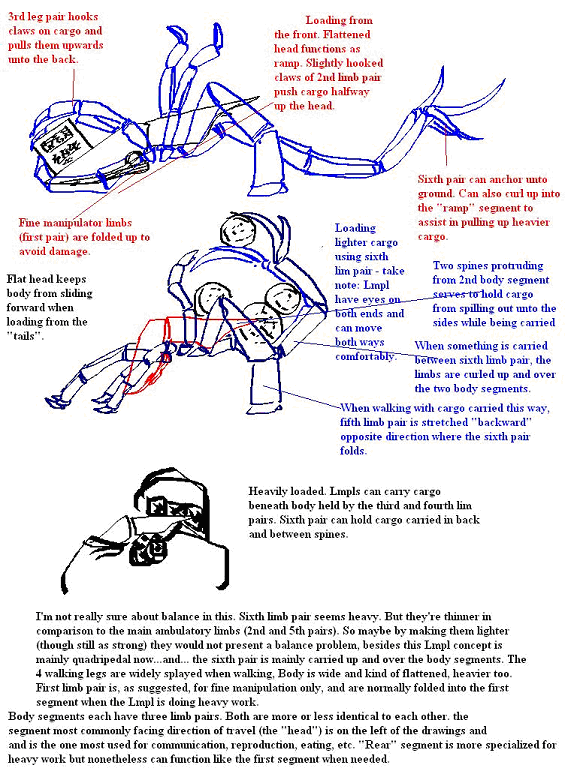
\includegraphics[width=0.75\textwidth]{../images/Lmpl-working.png}
}
    \caption{Lmpl doing work}
    \label{fig:Lmpl-working}
\end{center}
\end{figure}


\subsection{Habitat}
Oxygen-Nitrogen 

\subsection{Culture}
Like the Nuhln, the Lmpl were a sub-sentient species that the Rlaan
selected for uplifting. The Lmpl were a project in adapting a lifeform
to an envioronment inhospitable to Rlaan workers. The Lmpl are
intelligent, but remarkably, and sometimes to a fault, single-minded,
though such is in keeping with their technical workforce mission. The
second of the two major uplift projects, the Lmpl are considered a
solid success, and enjoy their own niche role in Rlaan
society. Admittedly, as they are Oxygen-Nitrogen breathers, they spend
very little time actually in Rlaan society proper.

\subsection{Religion}
All Lmpl are adherents of Rlaanbzztkrlbzeentkaan (see ~\ref{Rlaanbzztkrlbzeentkaan}). 

\subsection{Miscellaneous}
The Lmpl use Rlaan numbers. 

\section{Mishtali}

The Mishtali were the first intelligent life forms Humanity came in
contact with, and at the time were enjoying a prolonged and happy
bronze age. Perhaps fortunately for them, the Unadorned were the
discovering faction, governing the Mishtali with a benign neglect. The
Mishtali managed the jump from a nomadic existence to being spaceport
baggage handlers quite well, all things considered, only eating a
fairly small number of colonists and tourists in the process.

\subsection{Physical characteristics}
See Figures~\ref{fig:Mishtali} and ~\ref{fig:Mishtali1} for details.

\begin{figure}
\begin{center}
\makebox[\textwidth][c]{
    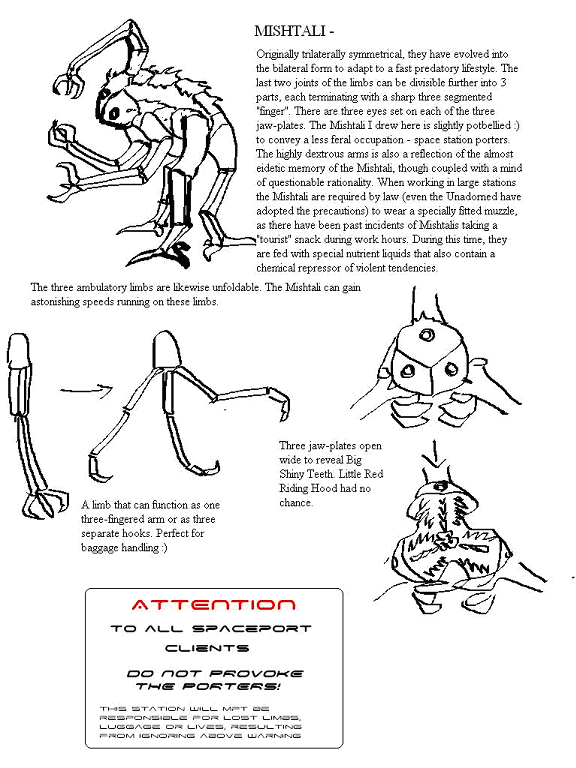
\includegraphics[width=0.75\textwidth]{../images/Mishtali.png}
}
    \caption{Mishtali}
    \label{fig:Mishtali}
\end{center}
\end{figure}
\begin{figure}
\begin{center}
\makebox[\textwidth][c]{
    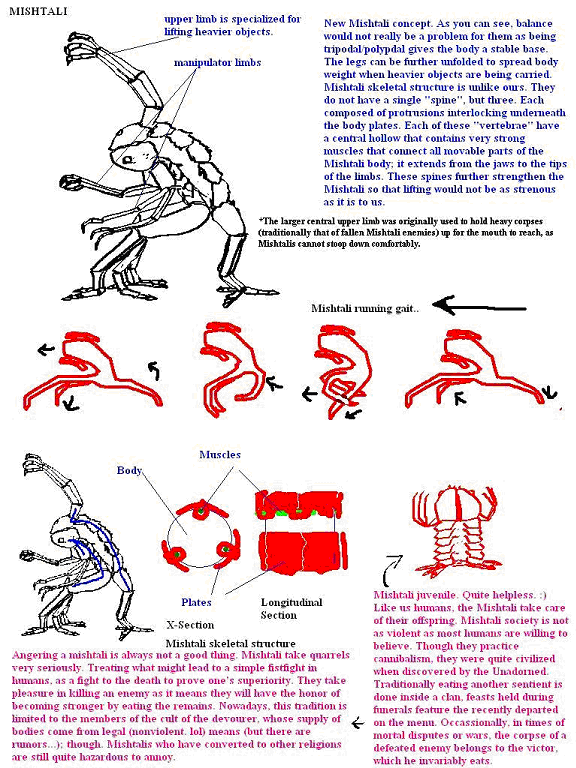
\includegraphics[width=0.75\textwidth]{../images/Mishtali1.png}
}
    \caption{Mishtali}
    \label{fig:Mishtali1}
\end{center}
\end{figure}


\subsection{Habitat}
Oxygen-Nitrogen FIXME 

\subsection{Culture}
Given the cultural oddities of both the Unadorned, who come close to
religious reverence in their views on computers, and the Mishtali,
known for being the source of the Cult of the Devourer wherein the
religious rituals are accompanied by the consumption of the remains of
both Mishtali and alien sentients, it is believed by many to be just
as well that the Unadorned, as their discoverers, are responsible for
shepherding them.

\subsection{Religion}

The Mishtali practice a number of religions, both native and
foreign. Chief among the native religions in, albeit infamous,
notariety, is the Cult of the devourer. The Cult of the Devourer
centers on the belief that success in life is directly tied with what
one eats, and that the more powerful the being that was eaten, the
better one's life can be. Thus, eating the remains of sentient beings
is as good as it gets. This, obviously, raises a few issues among many
groups, but there are enough humans and Dgn willing to be paid for the
eventual consumption of their corpse that the churches of the Cult of
the Devourer tend not to lack for sustenance. These churches are, as a
rule, very festive and pleasant places to visit, provided one is not
turned off by the cuisine. The Mishtali have been very willing to
convert to just about anything, so the Mishtali also tend to have the
largest alien populations of most obscure human religions.

\subsection{Miscellaneous}
Base e.

This is what happens when math types (of admitedly questionable
initial sanity) decide to bring civilization to an undeveloped species
that doesn't understand exactly what is meant by "optimal".

\section{Nuhln}

\subsection{Physical characteristics}
Figure~\ref{fig:Nuhln} provides a clear depiction of a Nuhln.

\begin{figure}
\begin{center}
\makebox[\textwidth][c]{
    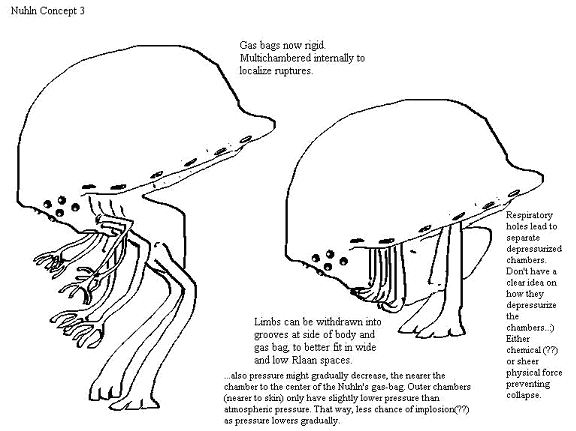
\includegraphics[width=\textwidth]{../images/Nuhln.png}
}
    \caption{Image of a Nuhln}
    \label{fig:Nuhln}
\end{center}
\end{figure}

 
\subsection{Habitat}
Methane-Nitrogen 

\subsection{Culture}
Like the Lmpl, the Nuhln were a sub-sentient species selected by the
Rlaan for an uplift project. The first of the two major uplift
projects, the Nuhln are generally considered far less successful than
the Lmpl, being somewhat intellectually slow. They are almost
exclusively found performing jobs where the ability to repeatedly
perform seemingly mindless tasks without complaint is a distinct
positive attribute. Though present throughout Rlaan inhabited space,
they are a culturally subsumed group, possessing no internal culture
to speak of.

\subsection{Religion}
All Nuhln are adherents of Rlaanbzztkrlbzeentkaan (see ~\ref{Rlaanbzztkrlbzeentkaan}). 

\subsection{Miscellaneous}
The Nuhln use Rlaan numbers. 

\section{Purth}

The Purth are an uplifted client species of the Andolians. In large
part an experiment in synthesis of work done by the Unadorned and the
Mechanists, the Purth are cybernetic beings, with assistive AI and
built in networking capacity. It is only through these upgrades that a
Purth achieves something much like sentience.  Although they sometimes
operate autonomously from their Andolian patrons, Purth never do so
alone. Only by networking their minds together will a group of Purth
be confident enough to venture off without guidance.

\subsection{Physical characteristics}
The Purth were chosen primarily because of their very hardy
constitution, and have proved themselves invaluable in high gravity
applications. Each individual Purth is quite large, comparable to a
small motor vehicles, and covered in a skin heavily composed of
silicones. The silicones are at their most present on the footpads,
which allow the Purth to walk across still-cooling lava flows and
traverse boiling mineral springs.FIXME

\subsection{Habitat}
FIXME 

\subsection{Culture}
FIXME 

\subsection{Religion}
The Purth were pre-sentient before the Andolians altered them, and are
universally predisposed to ignore religious issues entirely.

\subsection{Miscellaneous}
Purth use binary, due to their number processing being heavily
computer assisted.

\section{Rlaan}

Ammonia-blooded, methane breathers from a cool world distantly
orbiting a hot star, the Rlaan are a collection of oddities. Unique
among the known space-faring groups, the Rlaan are actually two
separate species, the defenders and workers speciating some hundred
thousand or so years ago.

\subsection{Physical characteristics} 
{\em (Defender, Workers and Hybrids)}

Rlaan are radialy symmetric beings with a base four
split. Figure~\ref{fig:Rlaan-perspective} shows a perspective view of
a Rlaan from above. Their Workers (see
Figure~\ref{fig:Rlaan-worker-cutaway}) stand about one meter high at
the prime knee, and are nearly one meter in diameter. Members of their
Defender caste (see Figure~\ref{fig:Rlaan-defender-cutaway} for
cutaway image of Defender species) tend towards being 50\% larger in
both dimensions. Rlaan natively breathe a methane-based atmosphere,
and must wear special breathing apparatus to negotiate oxygen-nitrogen
environments. Their skeletal structure, being an exoskeletal carapace
supported internally by millions of reinforcing struts, is best suited
to lower gravity worlds, and leads to the use of mechanical assistance
on larger or denser rocky bodies.

\begin{figure}
\begin{center}
\makebox[\textwidth][c]{
    
\includegraphics[width=3in]{../images/Rlaan-perspective.png}
}
    \caption{Rlaan - view from above and side}
    \label{fig:Rlaan-perspective}
\end{center}
\end{figure}
\begin{figure}
\begin{center}
\makebox[\textwidth][c]{
    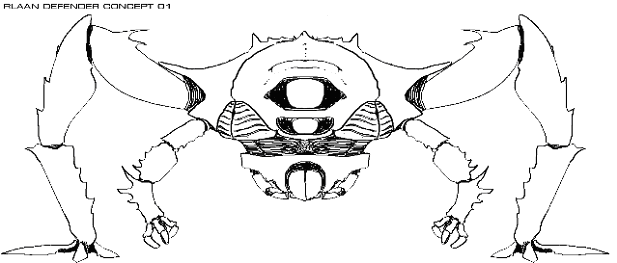
\includegraphics[width=\textwidth]{../images/Rlaan-defender-cutaway.png}
}
    \caption{Rlaan Defender - front and back limbs omitted}
    \label{fig:Rlaan-defender-cutaway}
\end{center}
\end{figure}
\begin{figure}
\begin{center}
\makebox[\textwidth][c]{
    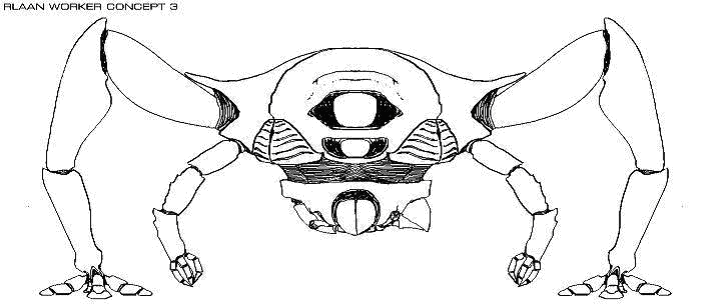
\includegraphics[width=\textwidth]{../images/Rlaan-worker-cutaway.png}
}
    \caption{Rlaan Worker - front and back limbs omitted}
    \label{fig:Rlaan-worker-cutaway}
\end{center}
\end{figure}

Both species are similar in appearance, with the primary differences
being size, the degree of fine control in the manipulator appendages
(workers have better fine control), and the structural integrity of
the skeleton (defenders are less fragile than workers).  The defenders
tend towards darker shades of red and purple, whereas the workers are
somewhat pale. Though the offspring of worker-defender matings are
sterile, these hybrids exist as nearly 4\% of the population, and have
come to play important social roles, especially in the realm of
politics.  Rlaan are radially symmetric with four equivalent
segments. Each of these segments contains one compound eye composed of
four segments, one ambulatory appendage, one mouth with four
mandibles, one manipulator appendage, various local organs, and
portions of the central organs. The Rlaan skeleton is a supported
exoskeleton, that is to say, the exoskeleton is supported internally
by a network of millions of small extensions of the skeleton, which
together form a sort of highly porous lattice that the soft internals
reside in. A defender stands about 1.5 meters high at the top of its
carapace, and 2 meters high at its knee joint. The central body is
around one meter in diameter, and a third of a meter in thickness. Out
of this central body come the four abulatory limbs, going up and out
from the body to the knee joint, and then proceeding down where they
terminate in a four-splayed gripping foot. Suspended below the central
body is the "head" portion of the Rlaan, about half a meter in
diameter and also about a third of a meter in thickness, with its
bottom covered in a particularly thick extrusion of the
exoskeleton. The manipulator appendages sprout from the region
connecting the head with the main body, and end in four radially
arranged fingerlike structures. A worker's dimensions are about 70\%
that of a defender.

\subsection{Habitat}
With equatorial temperatures peaking near 230 K, seas of ammonia, and
a methane atmosphere, the Rlaan homeworld is not what most species
would consider a prime vacation spot. Life on this planet progresses
at a rather slower pace than that on water worlds, but proceeds
nonetheless. From the point of view of ammonia-methane life, the Rlaan
planet is actually quite toasty.

\subsection{Culture}
Rlaan lifespans tend to be between 250-350 years. This is believed to
be a large factor in their cultural homogeneity and the methodical
nature of their advances, both through space and as a culture. Rlaan
culture itself is a very dry affair, with social dynamics primarily
involved around expository investigations of philosophical debates
that have yet to be satisfactorily translated into the language of any
other species.

\subsubsection{Music}

Their music, if it can be called such, has been compared to "the set
of frequencies one would expect to register if a Myztherian Octpanther
were let loose in a campanile". On a more disturbing note, the Rlaan
central archives possess the largest collection of data concerning
Jerry Lewis and Yoko Ono outside of Human space. The Rlaan are,
however, regarded by many of the other space faring races as much more
intelligent than their culture's taste in art would suggest.

\subsubsection{Writing}

Rlaan written language appears as a sequence of characters consisting
of one to four radial slashes in each of four quadrants formed by a
pair of crossed lines. It is read in a counterclockwise spiral out
from a blank central region that is reserved for the signature glyphs
of the author. The Rlaan have vast stores of written documents going
back thousands of years, but attempts to decipher most of them have
met with limited success, as the concepts often being discussed seem
to have no corollaries in the languages of any other species.

\subsubsection{Science}

Rlaan science is more advanced in the fields of chemistry and genetic
manipulation than any of the other space-faring races. The Rlaan are
also quite knowledgeable about materials science and the advances in
the latter are often related to the former. Aside from these noted
cases though, Rlaan science has advanced more slowly than that of the
Humans or the Aera, and the extent of its advances is more a measure
of the age of Rlaan investigations into science than any particular
brilliance on the part of the Rlaan. Though not truly uncreative, the
Rlaan seem hard pressed in the department of inventive spontaneity. In
particular, the Rlaan are rather behind humanity in their exploration
of both artificial intelligence and tightly integrated biomechanical
systems, having sufficed with loosely coupled designer organisms.

\subsubsection{Politics}

The Rlaan are governed by a body whose name translates to The Rlaan
Assembly it appears to be some form of representative democracy, but
the exact methods of choosing one's representative seem complex and
arcane beyond the tolerance of most observers to bother attempting to
figure out. This body then churns out laws and regulations at a
breakneck pace, the enforcement of which is then delegated to the
complex Rlaan Bureaucracy. Attempts to understand the inner workings
of the Rlaan Bureaucracy have met only with confusion for all parties
involved. Strangely, the members of the Assembly are
disproportionately sterile hybrids, believed by the Rlaan to be more
levelheaded than either the aggressive defenders or the timid
workers. One thing that did translate clearly, however, was the Rlaan
differentiation between civilian and non-civilian. Given their
biological distinction between these two, it is easy to see why the
Rlaan have such firm views upon how civilians should be treated.

Notable Rlaan Factions and Organizational Entities
\begin{itemize}
\item The Rlaan Assembly 
\item Rlaan Briin 
\item Rlaan Merchants 
\item Rlaan Hunters 
\item Rlaan Enforcers 
\end{itemize}
\subsection{Religion}
\label{Rlaanbzztkrlbzeentkaan}
Most Rlaan are adherents of Rlaanbzztkrlbzeentkaan. What this means is
very difficult to say, as, though it is a text based religion, the
text is under constant revision. Indeed, the Rlaan Assembly regularly
submits changes and additions to the holy text. Contradictory edicts
abound, and scores of companion volumes are included with every copy
that debate the relative merits of breaking one set of edicts over
another. Edicts contradicting each other,however, are the least of a
reader's worries, as the universe is created 37 times in 17 entirely
distinct fashions, by a grand total of 4301 entities, albeit 4210 of
these were all in one creation story. History, morality, ethics, and
the fundamental nature of reality itself are all presented in so many
different forms in the text, that it defies rational understanding as
to how the Rlaan consider the book canonical and relevant. However,
they do. And they gather together at one of the 73 specified intervals
of worship, for those that interpret worship as being allowed, to
engage in whatever activity is currently believed to be both correct
and legal by the group that has thus met. Rlaan places of worship are
thus remarkably like most Rlaan art: constantly changing in nature but
composed of themes that are themselves mind-numbingly repetitive, and
constantly possessed of an aesthetic that runs counter to common human
tastes.

\subsection{Miscellaneous}
Depending on your viewpoint, the Rlaan use either base 4 or base
256. Namely, every Rlaan character is composed of 4 subcharacters, so,
going by the subcharacters, it's base 4, but there are 256 distinct
numerals per character read. Rlaan numbers are distinguishable from
the characters in the rest of the Rlaan script in that the center of
each subcharacter is marked with a dot. As far as the Rlaan are
concerned, it's base 256.

\section{Saahasayaay}

Fast, beautiful and deadly, while they serve the Rlaan, they do so
because of the technological and economic benefits gained from the
association rather than out of gratitude. Whereas the Rlaan succeeded
in making both the Lmpl and Nuhln useful and docile, the Saahasayaay
are indeed useful, but far from docile.

While the Saahasayaay are a single species in the technical sense,
their array of different metamorphic forms, each clearly of distinct
origins, is somewhat unique, and, as only certain of the forms are
possessed of any particular intelligence, and only one of accepted
sapience, in common reference "Saahasayaay" may often refer only to
the portion of the population in dominant sentient morphology.

The Saahasayaay have the strangest, and, on several levels, most
disturbing life cycle of any of the known extant sentients. Foremost
among its disturbing points is that the life cycle is clearly of
artificial origin external to the Saahasayaay homeworld. The
non-squeamish often find this more disturbing than the fact that
metamorphosis usually begins with the death of much of the body, and
proceeds via the semi-autonomous archival organ consuming what would
otherwise be the uneaten remnants of its own corpse to fuel its
generation of a new body. The archival organ, itself effectively
inedible, and encased in a protective shell, is not a native
feature. The organ features an absurd amount of unexpressed genetic
code - indeed, it contains genes describing thousands of species,
almost none of which are actually present on the Saahasayaay
homeworld. Indeed, the Saahasayaay appear to be the result of some
ancient (although not believed Ancient) xenoforming gone awry. Many of
the gene sequences present in the archival organ appear to be
irrevocably damaged or woefully incomplete, despite the presence of
significant error correcting facilities.

Only the lowest level of the metamorphic chain for the Saahasayaay can
actually breed. All other forms have been rendered sterile. This
lowest level is a fast growing photosynthetic invader species that has
infiltrated or replaced competitors in most of the native ecosystems
of the Saahasayaay planet. It cannot be correctly termed a plant,
animal, or fungus, although it shares some features with all of these
more familiar categories. While likely originally designed to be the
prime xenoforming agent for the planet, destroying native ecosystems
and replacing them with those of its creators, the archive creeper has
wandered from its original mission, producing a warped hybrid
ecosystem that almost certainly bears little resemblance to either the
original or intended replacement. The origins of the Saahasayaay are
clear in both their metamorphic paths, their traditional food chains,
and the sterility and monosexual nature of all of the extant forms
save for the archival creeper. Local "herbivores", for lack of a
better word, came to eat the creepers, but were in turn recorded and
replaced, themselves devoured and recreated by the archival organs
they attempted to consume. This effect then proceeded to trickle up
the food-chains of all of the ecosystems invaded by the creepers. A
limitation of this process, was, of course, that organisms smaller
than the archival organ were not readily assimilated. Thus, the
detritus feeders competing for flesh on the fallen corpse of an
assimilated species were more likely eaten by the archival organ than
the other way around.

The archival organ is an incredibly complex, advanced, and subtly
broken biological machine, but it is not itself remotely
intelligent. Likewise, it is not quite sufficiently autonomous to
generate widespread agreement as to it being referred to as a
symbiotic organism, especially as the genetic definitions are skewed,
given that it contains all of the genetic code for all of the "host"
bodies. All tissues in the archival organ feature cellular
immortality, and the archival organ is itself amortal (not aging, nor
dying from old age) although the bodies it produces do not share these
properties. The organ is well protected and possesses some independent
subsystems, so surviving the death of the rest of the body is common
(depending on the manner of host-death) - which is necessary, given
that such is the only means for morphological change and the
preservation of more interesting forms of species. The archival organ
plays key hormonal regulatory roles in all of the assimilated forms.

\subsection{Physical characteristics}
Terminal form Saahasayaay are physically impressive beings, if not,
because of mode of movement, as bulky as some of the other sapients,
and fossil records indicate this to be a quality preserved from
pre-assimilation times. They are beautiful, if possessed of features
that, if designed, would speak of a certain viciousness to the
crafting hand. The terminal Saahasayaay are the only extant sophonts
known to be able to fly, albeit they are, in practice, more often
gliders than active flyers through their thick and caustic
chlorine-nitrogen atmosphere. Their bodies are long, almost
serpentine, though the strong muscular development for the wings and
arms belies that image. They are bilaterally symmetric, with 4 wings
rising above, and 8 arms hanging below the largest and middlemost
segment of the body, set between a long tail at rear and longish neck
and fierce head at front. The front and rear sets of arms have
hand-like endings, gripping appendages of a gaunt leather-and-bone
appearance, that are dexterous, if clearly meant to hold fast to live
and struggling prey while the curved blade-like endings of the middle
four arms carved and scooped the meal into edible submission. Skin on
the middle-body is mostly hidden behind large, thin, overlapping
scale-like protrusions of smooth, hardened flesh, iridescent, ranging
through colors from green to red to gold. The tail, in cross section,
could be thought of as a square whose sides have been bent in, or
whose corners were pulled out, to produce a four-sided concave
shape. The tail is heavily segmented, as is the neck, which has a
similar shape, although much larger, and it lacks the short spines
protruding from the corners of each tail segment that serve to let the
tail be used to grip surfaces or objects it has been wrapped
around. The tail narrows somewhat as it progresses rearwards, but was
always fairly thin in comparison with the body. Towards the rear of
the tail, the spines end, and four specialized spines are present that
act as fins that can be raised or lowered to act as flight control
surfaces. The scale-like protrusions are much larger on the tail and
neck than on the body, corresponding heavily to the structure of the
segments themselves leaning somewhat towards a more chitinous-plates
appearance than scale-like appearance, for those portions, although in
truth it is only a matter of size and flexibility required for each
segment that has lead to the differing appearance, and not a
fundamental change in material. The head is slightly larger in girth
than the neck, excepting the mouth itself which is forward of the rest
of the head. The terminal form Saahasayaay have no teeth in their
mouth. Grinding, separating and pulverizing are instead done by
stone-hard protrusions that line their equivalent of the
esophagus. The mouth instead consists of a set of flexible, segmented
spines, connected to each other by membranes, that can be focused to a
point, as when sucking in fluids or flying, or opened to engulf a
portion of a prey animal. This semi-engulfing is necessary, as the
chunks of flesh freed from the target by the multiple bone-bladed
tongues that slash out violently from within the mouth might otherwise
fall out. There are four eyes, two at the corners of the top of the
head and two, more centered, below. There are ears and nasal openings
that lie on the side of the head. The brain itself is primarily on the
top of the head, although there is significant neural matter at the
bottom of the head that does optical processing for the lower eyes.


\subsection{Habitat}
All of the native species integrated by the archival organ are now
extinct. Thus, entire food-chains now consist of nominally Saahasayaay
organisms. It is presumed, given that all of the non-creeper
morphologies are sterile, that the intended process involved a
kill-off of all of the food-chains via a wave of progressive
morphology changes up the food-chain, thereby progressively starving
each link in the chain. Alternate theories presume an external agent
being introduced that would kill off all of the hybridized life forms,
while leaving the invaders intact, but the non-native codes are
sufficiently mangled that it has been difficult to test if such
differentiation would have been readily achievable. Given the large
number of codes stored, it is presumed that total kill-off was not an
intended goal. Clearly, however, none of these have happened,
especially those models requiring external intervention. Instead, the
regulatory mechanisms presumably in place to delay any native
depopulation until there has been sufficient infiltration of the
native populations have instead functioned merely to regulate the
frequency with which the next body of a dead Saahasayaay differs from
the previous. Also noteworthy is the terminal nature of the
Saahasayaay metamorphic process. Fossil records point to the ancestor
of whatever native species preceded the sapient Saahasayaay population
as having been wide-ranging, and wherever present, atop the food
chain. Thus, the Saahasayaay sophonts are currently the "terminal"
metamorphic form - an archival organ that survives a Saahasayaay
sapient's death will normally build another Saahasayaay sapient. Note
that none of the previous individual's memory or mentality is
preserved, and inefficiencies in conversion and the genetic
imperatives of brain development in the original source species, even
in the presence of a nearly full corpse, result in the production of a
juvenile individual.


\subsection{Culture}

The most successful of the Rlaan client species, the Saahasayaay are
not, unlike the Nuhln and Lmpl, true uplifts, having already achieved
some minimal level of societal advancement at the point of discovery.

The Rlaan have taken to using Saahasayaay troops to reinforce their
border with the Aera, are, however, somewhat hesitant to let this
concentration of troops return home.

As most of the Saahasayaay forms are not capable of complex thought,
they don't much consider either the nature of their life cycle, nor
that they often are eating what is technically a member of their own
species. This is not the case for terminal form, whose culture has
been deeply shaped by the role that death plays in the Saahasayaay
life-cycle, and the semi-reincarnations that are the daily occurrences
of Saahasayaay life. The terminal form Saahasayaay are, in fact, quite
bright, and learn voraciously, but a cultural disinterest in knowledge
unrelated to superior killing ability and an exceptionally low
life-expectancy rate due to unending war, murder, and ritual killings
has historically hampered internal sources of advancement. It is not
too difficult to see where their obsession with death has come from,
albeit only they, perhaps, can truly comprehend the directions it has
taken them in. It is fortunate for all other sapient species in the
region that the Saahasayaay were found in the stone-age by
space-faring sapients, and not the other way around, as the
Saahasayaay have no compunction when it comes to killing, whether it
be other sentients, each other, or lower Saahasayaay forms. Death is
the natural order for them, it is the source of progress, and their
right and duty to disperse. Their obedience to the Rlaan and restraint
in aggression against both the Rlaan and other species is predicated
on the Rlaan's greater ability to bring death upon them than they upon
the Rlaan, as well as the opportunity for greater empowerment that the
Rlaan bring to the Saahasayaay. Death is the ultimate blessing the
Saahasayaay believe they can bestow, and the frequent regeneration of
their fallen into newborns has utterly deprived them of the fear of
their own demise present in all other known organized species of
measurable intelligence.

Some of the other Saahasayaay forms possess some level of
intelligence, though none as pronounced as the terminal form
Saahasayaay. Some of these forms have been "domesticated" and the most
intelligent of these, generally considered comparable to some of the
Terran primates, are sometimes used in a servitor role. The most
valued of the servitors are granted a chance at "ascension" by being
taken to an isolated area, free of terminal Saahasayaay, and killed
swiftly, leaving the entire corpse intact. The lack of terminal
Saahasayaay in the area improves the likelihood that the next
metamorphic form will be a terminal Saahasayaay, rather than another
servitor, as the choice of next form is heavily influenced by the
presence of other forms detected by the archival organ, a
manifestation of its original, more overarching regulatory
role. Punishment in terminal Saahasayaay society rarely involves
killing of the archival organ, an act considered disgraceful unless
the individual in question has been deemed to be heretical to the
advancement of the Death God's agenda, but it almost universally
involves killing. Punishments range from the minor, a swift and clean
death followed by adoption for what most other species would consider
misdemeanors, to use as hunt bait and eventual consumption by lower
forms, to the most serious crimes being punished by the removal of the
archival organ, the starvation thereof for a period of time, to
increase the chance of form reversion, smearing the archival organ in
the mixed remains of lower forms to further increase the odds that the
next form will not be a terminal Saahasayaay, and then letting the
starving archival organ eat the victim (still conscious, but wracked
with crippling chemical imbalances) alive.

It is generally considered fortunate that only a small percentage of
the world known to be reachable via the jump network feature a
chlorine based ecology. The Saahasayaay, from the creeper on up,
feature a profoundly rapid metabolism, and they have quickly overrun
and populated other chlorine-worlds that they have been introduced
to. Indeed, it has long perplexed researchers as to why exactly the
concentration of chlorine-life friendly worlds is significantly higher
in the region of space containing the Saahasayaay homeworld, and then
marginal elsewhere. What many believe to be the likely originating
planet of the archive creeper is in very nearby space, just one jump
link removed from the Saahasayaay system, but it is difficult to
ascertain this connection with any certainty. The system shows signs
of previous habitation by a technological entity, but, outside of
semi-preserved ruins on various moons and other uninhabitable
locations, there is precious little left of the inhabitants. In
particular, what is believed to have been their homeworld would seem
to have fallen victim to both some sort of limited grey-goo event and
a widespread use of fusion, antimatter, and kinetic weapons that,
combined with the already reactive nature of the atmosphere, served to
make it exceptionally difficult to discern much about the previous
inhabitants. Levels of nano-plague are also exceptionally high in the
system, leading several researchers to advance theories that the
inhabitants made what proved to be a fatal mistake of attempting to
counter the nano-plague in an aggressively military fashion.

The Saahasayaay navigate 3D space with great agility, and, despite the
distinctly different dynamics of planetary and vacuum flight, make
excellent pilots in either medium. The Saahasayaay have not
significantly industrialized on their own, although their
technological usage has greatly advanced since absorption into the
Rlaan Assembly. All Saahasayaay ships are specially manufactured for
them by the Rlaan out-system, and Saahasayaay pilots shipped out to
military bases from one of the Saahasayaay worlds. The Rlaan are
somewhat reticent when it comes to providing the Saahasayaay with a
means to make their own starships. They are, however, more than
willing to freely give them technologies which increase their
sustainable populations so that they can draw upon more Saahasayaay
troops. The Saahasayaay, for their part, hunger for more control over
their own destiny, but are currently kept sated with the opportunity
to bestow much bigger deaths with the starships the Rlaan build for
them (the Saahasayaay consulting on certain aspects of the
design). Saahasayaay operating in Rlaan space must wear
atmosphere/temperature suits at all times, precluding flight
abilities. Their suits are therefore augmented with thrusters so as to
make them more comfortable - an uncomfortable Saahasayaay is not a
safe Saahasayaay, though there is of course, no such thing to begin
with. Saahasayaay work only with defenders and hybrids in Rlaan
society. They have no respect for the Rlaan workers, who cannot be
killers in any meaningful way, and the Saahasayaay are considered an
unnecessary threat in interacting with Rlaan workers.

\subsection{Religion}
The dominant belief structure of the Saahasayaay revolves around each
of them being an intruments of the great death god who sits in
judgment over the universe. The Saahasayaay belive themselves to be
the chosen people who alone are privy to the sentences being passed
down upon the mortals of this realm. Saahasayaay prophet halls are
built to express the joy of the hunt, the glory of the kill, and
subserviance to the great death god. The prophet halls are built in
keeping with the 3-dimensional nature of Saahasayaay travel, with
perches on many levels, and rank denoted by attainment of a higher
perch.

\subsection{Miscellaneous}
The Saahasayaay used to use a unary system with groupings done in sets
of 8 (flat, without a notion of base), but have been converted to use
of the Rlaan base 256 system.

\section{Shmrn}
\label{subsec:Shmrn-species}
The Dgn and Shmrn share a common time-of-uplift ancestor. The
resulting species was further refined in seperate efforts by the
Lightbearers and the Shapers into two distinct, but closely related
species. As the Lightbearers were destroyed as a meaningful entity,
the Shmrn were let loose as a freed species to settle new worlds.

\subsection{Physical characteristics}

\subsection{Habitat}

\subsection{Culture}

For above 3 categories, please see the following list of images: Figures \ref{fig:Shmrn-overview}, \ref{fig:Shmrn-ancestral}, \ref{fig:Shmrn-elder}, \ref{fig:Shmrn-medic}, \ref{fig:Shmrn-pilot}, \ref{fig:Shmrn-pilot1}, \ref{fig:Shmrn-footwear}, \ref{fig:Shmrn-formalwear}, \ref{fig:Shmrn-logo}, and \ref{fig:Shmrn-render}.

\begin{figure}
\begin{center}
\makebox[\textwidth][c]{
    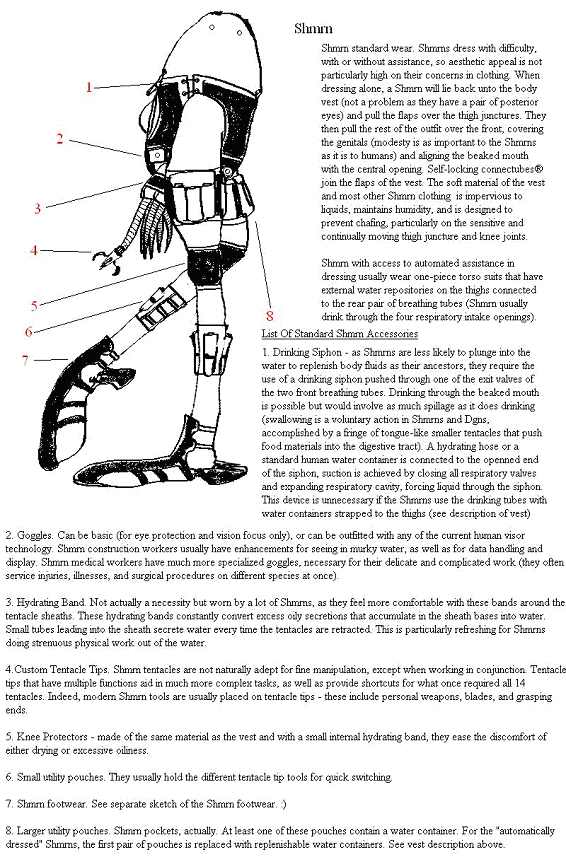
\includegraphics[width=0.75\textwidth]{../images/Shmrn-overview.png}
}
    \caption{Shmrn Overview}
    \label{fig:Shmrn-overview}
\end{center}
\end{figure}
\begin{figure}
\begin{center}
\makebox[\textwidth][c]{
    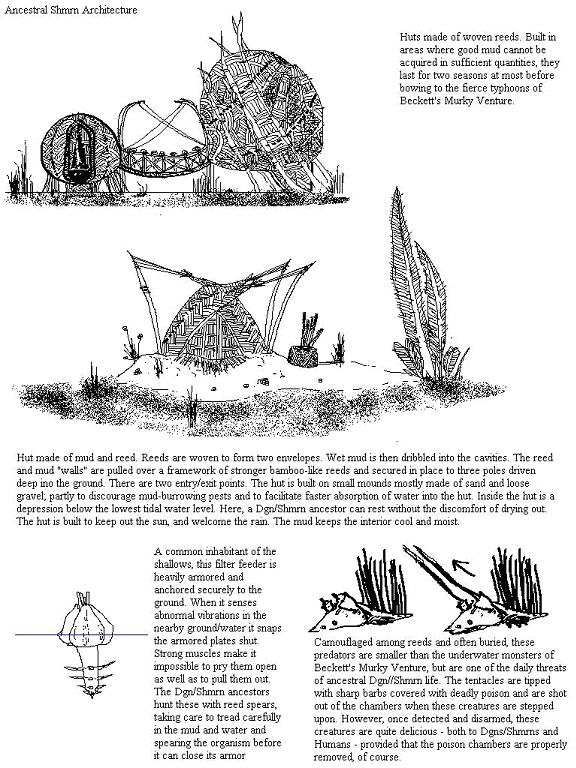
\includegraphics[width=0.75\textwidth]{../images/AncestralShmrnArchitecture.png}
}
    \caption{Habitat of the ancestral Dgn/Shmrn}
    \label{fig:Shmrn-ancestral}
\end{center}
\end{figure}
\begin{figure}
\begin{center}
\makebox[\textwidth][c]{
    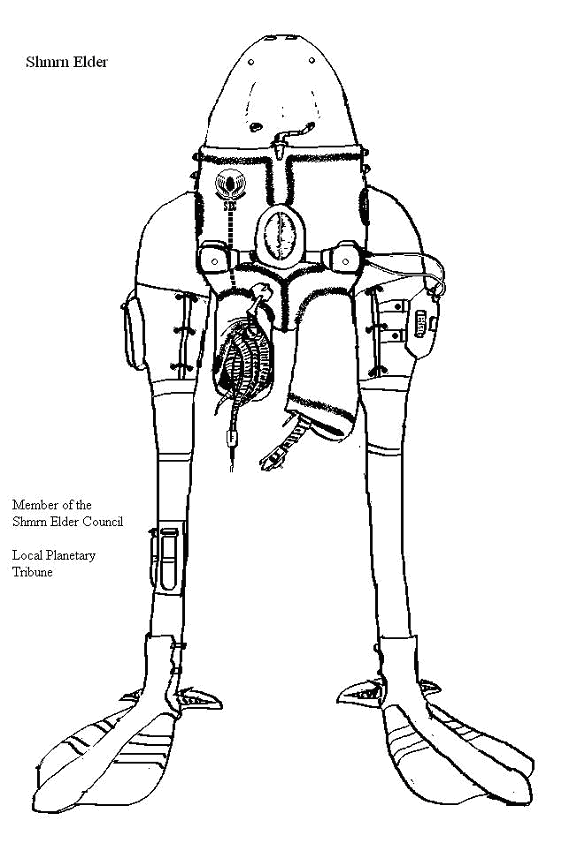
\includegraphics[width=0.75\textwidth]{../images/Shmrn-elder.png}
}
    \caption{Shmrn Elder}
    \label{fig:Shmrn-elder}
\end{center}
\end{figure}
\begin{figure}
\begin{center}
\makebox[\textwidth][c]{
    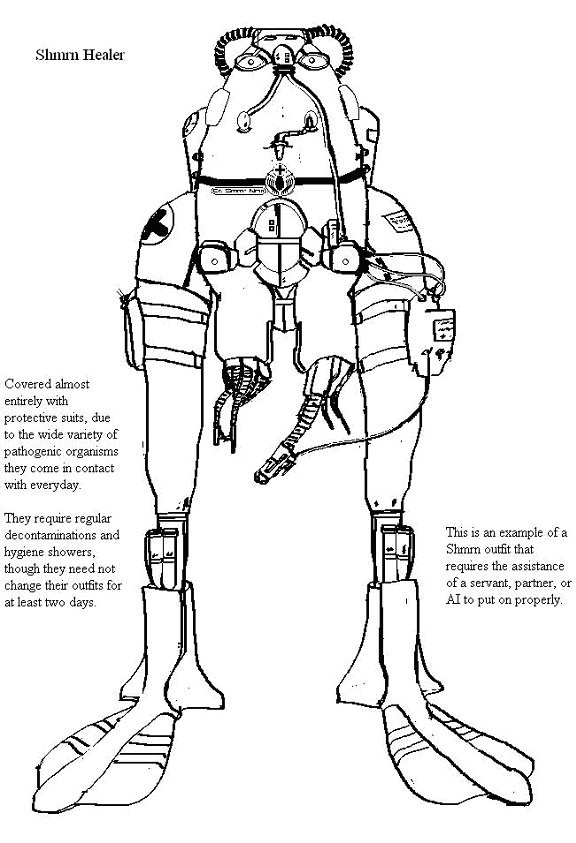
\includegraphics[width=0.75\textwidth]{../images/Shmrn-medic.png}
}
    \caption{Shmrn Medic}
    \label{fig:Shmrn-medic}
\end{center}
\end{figure}
\begin{figure}
\begin{center}
\makebox[\textwidth][c]{
    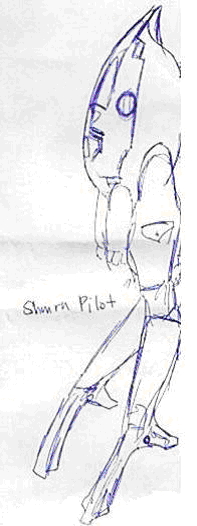
\includegraphics[width=0.25\textwidth]{../images/Shmrn-pilot.png}
}
    \caption{Shmrn Pilot(1)}
    \label{fig:Shmrn-pilot}
\end{center}
\end{figure}
\begin{figure}
\begin{center}
\makebox[\textwidth][c]{
    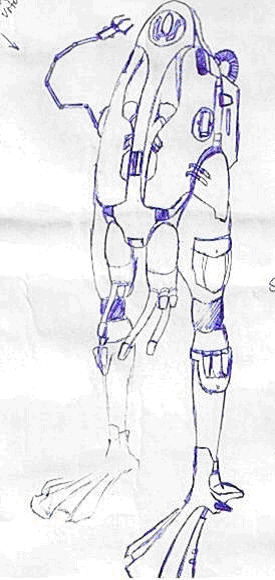
\includegraphics[width=0.25\textwidth]{../images/Shmrn-pilot1.png}
}
    \caption{Shmrn Pilot(2)}
    \label{fig:Shmrn-pilot1}
\end{center}
\end{figure}
\begin{figure}
\begin{center}
\makebox[\textwidth][c]{
    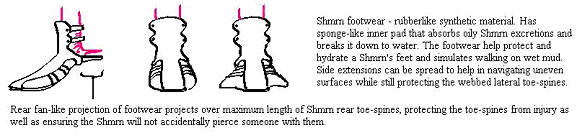
\includegraphics[width=\textwidth]{../images/Shmrn-footwear.png}
}
    \caption{Shmrn footwear}
    \label{fig:Shmrn-footwear}
\end{center}
\end{figure}
\begin{figure}
\begin{center}
\makebox[\textwidth][c]{
    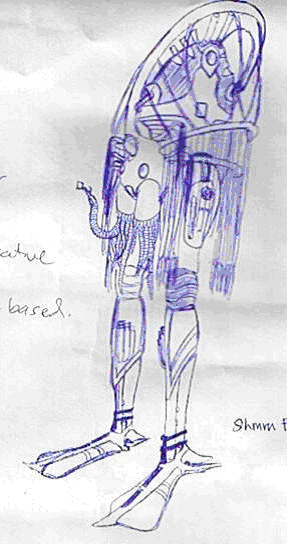
\includegraphics[width=0.5\textwidth]{../images/Shmrn-formalwear.png}
}
    \caption{Shmrn formalwear}
    \label{fig:Shmrn-formalwear}
\end{center}
\end{figure}
\begin{figure}
\begin{center}
\makebox[\textwidth][c]{
    
\includegraphics[width=2in]{../images/Shmrn-logo.png}
}
    \caption{Shmrn logo}
    \label{fig:Shmrn-logo}
\end{center}
\end{figure}
\begin{figure}
\begin{center}
\makebox[\textwidth][c]{
    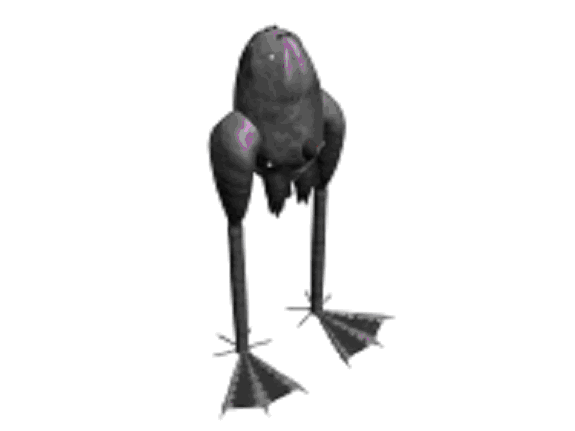
\includegraphics[width=\textwidth]{../images/Shmrn-render.png}
}
    \caption{Shmrn - rendered}
    \label{fig:Shmrn-render}
\end{center}
\end{figure}

\subsection{Religion}
The Shmrn have a spiritual existence quite different from their
brothers the Dgn, with communal meetings contemplating the nature of
suffering over one's lifetimes dominating the organized religious
landscape. Shmrn culture and universe view centers on the principles
that life is unfair and painful, but a necessary stage to receive the
reward of eternal painlessness that awaits those who have, over
several lifetimes, overcome their desires to avoid the unpleasantness
of life.

\subsection{Miscellaneous}
Base 7. Nothing special. 

\section{Super Cetaceans (SuCets)}

Super Cetaceans (SuCets) are the result of what some consider the
first truly profound endeavours of Humanity in combining the fields of
genetics and cybernetics. While there are still SuCets around, they
are generally considered a "failed" experiment, never thinking in a
sufficiently compatible manner to become either useful tools or
partners, and requiring cybernetic additions that were too costly,
post nano-plague, for novelty value. Small communities of SuCets exist
on some of the more affluent and metropolitan oceanic worlds, and
their largest community, though quite small, remains on Earth.

\subsection{Physical characteristics}
The bulk of their genetic code derived from a potpourri of whales and
porpoises, they are oxygen breathing swimmers of immediately
recognizeable cetacean form, overcoming their lack of manipulator
limbs via integrated mechanical prosthesis.

\subsection{Habitat}
The shallower seas of the continental shelves and the vast waters of
oceans and oceanic worlds with oxygen-nitrogen atmospheres.

\section{Super Simians (SuSims)}

Super Simians (SuSims) and SuSim Cyborgs have been one of the more
stunting trends for "true" AIs, arising from the advances in the
fields of genetics and integrated cybernetics. For physically
manifested tasks considered too menial, too dangerous, or too
monotonous for Humans, the SuSims and SuSimCys proved cheaper, more
reliable, and, through advancements in genetics, easier to dominate
than AI alternatives.

As a client race they are quite prevalent in High-Born space as
servants. In other societies, however, the use of SuSims is seen as
inhumane or otherwise frowned upon.

\subsection{Physical characteristics}

The SuSims were constructed from augmented blends of Terran primates,
and many discernable features of their Chimpanzee and Bonobo ancestors
are immediately recognizeable. They remain hairy, not for practical
purposes, as much as to help convince their masters that the lines
between pet, tool, and slave have not been crossed in an era when some
"Humans" may be further distant genetically than the SuSims are from
Homo Sapiens Sapiens.

\subsection{Habitat}
They are capable of breathing an oxygen-nitrogen atmosphere. 

\section{Those who have only names (TWHON)}

What little is described of this group is gleaned from writings left
behind by the Ancients. While most descriptions are quite vague, it is
clear that TWHON, if the Ancients are a reliable source, were at least
as advanced as the Ancients, and much older.

\section{Uln}

FIXME 

\subsection{Physical characteristics}
 
8 limbs, 4 legs, 4 arms. Each arm end in a "hand" with 4 "fingers" one
of which is opposable. The four legs terminate in fleshy-padded feet,
each of which ends in sets of broad, thick, fore and back claws
capable of allowing "tree"-climbing. All four legs are visible in the
rear picture (this specimin has somewhat skinny front legs). The two
arm pairs are socketed between the two leg pairs, one pair of arms
reaching over the head, the other coming up from under. The head is
large and block-like, situated on a short, muscular stalk of a neck
protruding from the main torso. The main torso features twin rows of
breathing holes, visible on the back/underside.

There are 3 moving parts in the Uln jaw, a lower jaw, and two side
portions, all of which are normally involved in eating. There is a
single visual input band that stretches across the front and onto the
sides of the Uln head, forming a cover for their complicated compound
eye. Uln vision is actually remarkably good, and they can see from the
infrared/near-microwave into soft UV (hence, some interesting trends
in Uln clothing materials).

Figure~\ref{fig:Uln-bodyplan} sketches the basic shapes described above.

\begin{figure}
\begin{center}
\makebox[\textwidth][c]{
    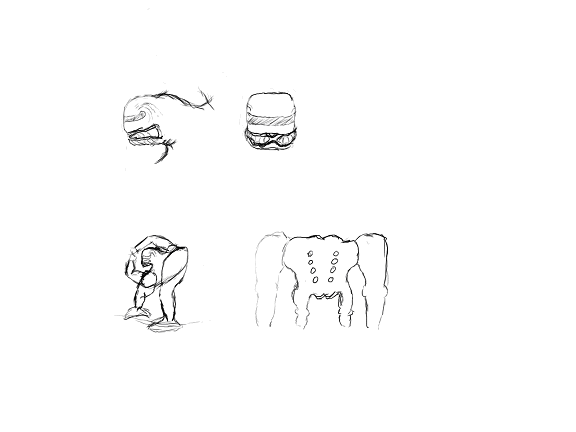
\includegraphics[width=\textwidth]{../images/Uln-bodyplan.png}
}
    \caption{Partial sketches of Uln body plan, details of head.}
    \label{fig:Uln-bodyplan}
\end{center}
\end{figure}


\subsubsection{Digestion}

The Uln don't do well with carbonated beverages. At all. Their
digestive tract isn't suited to things that expand that rapidly upon
consumption, and they will make a horrid, stinky mess of things when
they exhibit that gem of convergent evolution (traditionally for toxin
removal) of spewing their food back out.

\subsection{Habitat}
FIXME 

Oxygen-Nitrogen.

       (Shmrn logo)


\subsection{Culture}
The Uln culture sprang up among the remains of a sprawling set of
Ancient structures and advanced in technology faster than their
biology or social structures could adapt, leading one noted human
researcher to note upon seeing them, "It was as if I had suddenly come
across a spacecraft piloted by Homo Erectus -- if they hadn't been so
ill prepared for the gifts they unintentionally received, they would
have conquered the entire arm." Fortunately for the aspirations of
dominance held by other species, the Uln were decidedly
unprepared. Indeed, they spent so much time blowing each other up with
weapons they didn't entirely control that it is a wonder that either
they or the ruins on their planet still survive.
\begin{itemize}
\item History

Uln development is somewhat difficult to follow, as they are not
actually "native" to their homeworld. Indeed, very little of the plant
and animal life on the entire planet appears to have been of native
origin, present for only millions of years. In particular, the species
on the planet appear to have come from many different origins, as is
sensible given the broad range over which Ancient sites have been
discovered in other star systems. The Uln are not generally very
talkative about their origins, especially as it is the common
agreement among the other sapients that they're the descendents of
whatever the Ancients were using for lab rats/monkeys. It is therefore
still a matter of some debate as to which features of the Uln are
naturally occurring, which were engineered, and what reasons there
were for such choices.

\item Clothing

The most commonly worn Uln garments range from "open-toed(clawed)"
short-boots, some utility pouches with straps around the upper arms
resting on the neck, and a helmet-scarf (draping down to cover more
sensitive regions between the underside of the neck and the lower
arms) which would be common casual-wear for the common peon, to the
foul-weather knee-length boots and helmet-poncho and the bizzare
extravagances of the aristocratic class, with gaudy creations not
unlike wearing an array of very fine wire-meshes and doilies, that
require servants to dress them. The back/underside is not normally
overly covered, though something may drape loosely behind the top arms
- to do otherwise would interfere with their breathing.
\end{itemize}
\subsection{Religion}
Growing up amidst the ruins of an exceptionally powerful and ancient
culture on a planet where life was artificially introduced gave the
Uln the idea that they were the children of failed gods. Convincing
them that they are much more likely the descendants of
lab-monkey-analogs from a long destroyed outpost hasn't gotten very
far. What passes for organization in Uln religion involves seasonal
festivals that mostly serve to reinforce the doctrinal line that being
born Uln is a wonderful thing, relative standard of living to the
other species be damned.

\subsection{Miscellaneous}
Base 4. Nothing special. 
